\chapter{Conclusioni}
\label{chap: Conclusioni}

\section{Introduzione}
Durante lo studio di fattibilitá e il successivo sviluppo, abbiamo constatato che le potenzialità del Dial in ambito industriale sono molteplici, dal miglioramento della User Experience alla precisione adottata nell’utilizzo.
Grazie al DialService è stato possibile trasferirle anche in ambito web, in quanto all’interno dell’impresa Loccioni sono presenti moltissimi settori in cui il Dial migliorerebbe molto l’esperienza utente e porterebbe una diminuzione di tempi e costi.\\ \\
Al momento dello sviluppo, la necessitá di dover passare per un applicazione UWP rappresenta sicuramente una limitazione che andrá tolta qualora il progetto verrá rilasciato in maniera industriale.
A favore di questa critica, nel mese passato, la Google stessa ha rilasciato in fase di Preview una libreria Web chiamata Trial for WebHID, la quale permetterá di far comunicare direttamente con la pagina Web i dispositivi che utilizzano il protocollo HID, come il Dial, permettendo agli sviluppatori futuri di non dover necessariamente passare attraverso una WebView o una applicazione nativa per quel dispositivo.\\

\begin{figure}[htpb!]
\center
  \includegraphics[width=0.2\textwidth]{Potenziometri}
  \caption{Potenziometro utilizzato attualmente}
\end{figure}

Nel nostro caso, l’utilizzo finale del Dial nei banchi prova del gruppo Loccioni, comporterebbe una maggior sicurezza in termini di precisione nella variazione di dati, in quanto al momento vengono utilizzati dei semplici potenziometri con le evidenti limitazione che essi comportano, come ad esempio la presenza di un inizio e fine corsa del potenziometro stesso, l’assenza di feedback durante l’utilizzo, la limitata corsa e di conseguenza la necessaria approssimazione dei singoli step eseguiti.

\begin{figure}[htpb!]
\center
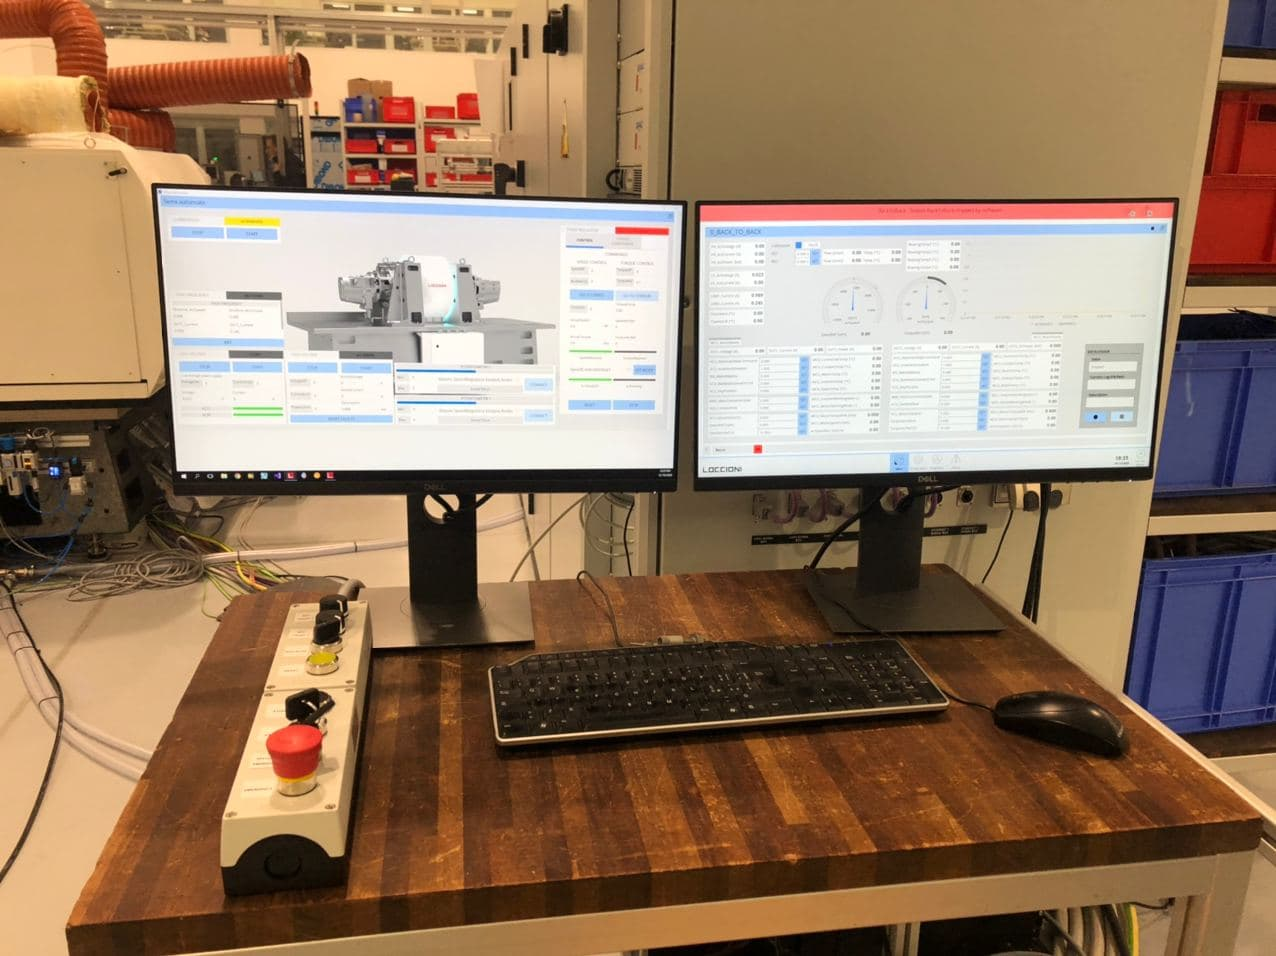
\includegraphics[width=0.2\textwidth]{Postazione}
\caption{Potenziometro utilizzato attualmente}
\end{figure}

Queste problematiche verrebbero risolte attraverso il Dial, in quanto presenta una “corsa” illimitata, un feedback atpico personalizzabile in base alle operazioni che si svolgono, una precisione laser a 3600 punti e la possibilitá di interagire direttamente con lo schermo, appoggiando il Dial su di esso, permettendo quindi una serie di combinazioni di utilizzo estremamente vasta.
\section{Sviluppi Futuri}

I possibili sviluppi sono molteplici e un’idea iniziale è quella di inserire un nuovo widget all’interno della dashboard Loccioni in grado di raffigurare attraverso un’immagine una parte del motore o elemento da controllare, in modo tale da avere un’interfaccia più intuitiva per la selezione, e poi, una volta selezionato il widget stesso, avere la possibilità di visualizzare i dettagli del componente attraverso il menù del Dial.\\
Una seconda modifica da apportare agli widget esistenti è sicuramente quella del controllo del moltiplicatore da applicare ad ogni rotazione avvenuta con il Dial, portando così maggiore precisione nei lavori più complessi e anche rapidità di utilizzo nelle parti che necessitano più rotazioni di Dial.\\
Uno sviluppo futuro sicuramente necessario è l’aggiunta di un controllo sui dati in input lato web, che momentaneamente non è presente nei nostri widget, ma è fatta solamente lato backend.\\
Per aumentare l’utilizzabilità dell’interfaccia utente è sicuramente necessaria una modifica degli widget da noi creati, per renderli più facilmente selezionabili dal Dial e per migliorare anche l’aspetto visivo.
In caso poi il progetto arrivi al punto di essere utilizzato, per migliorare la manipolazione di dati in uso nelle dashboard attuali è necessario sicuramente apportare alcune modifiche alla dashboard per consentire un utilizzo attraverso il touchscreen di un qualsiasi dispositivo, in modo tale da rendere veramente fluido l’utilizzo di tutto l’ambiente e poter così eliminare il mouse dalle operazioni svolte più frequentemente.\\
Per concludere, un possibile miglioramento da apportare al codice è quello di una selezione più veloce ed accurata del widget attraverso il posizionamento sullo schermo, magari attraverso un movimento anticipato del mouse o un movimento continuo.
\section{Considerazioni}

\section{Evoluzioni dell'Art of State}

%SULLE CONCLUSIONI

Una volta avvenuto il caricamento della pagina Web nell'applicazione UWP, ci rimaneva da risolvere il problema della comunicazione tra due linguaggi differenti, quello Web, nel nostro caso, basato sul TypeScript e quello UWP interamente in C e XAML.\\

Le comunicazioni dovevano avvenire in maniera bi-direzionale, questo significa che non é solamente l'applicazione UWP a comunicare con la pagina Web, ma anche viceversa. Affinché l'applicazione potesse comunicare con la pagina Web, grazie alla funzionalità InvokeScriptAsync, messa a disposizione dalla WebView, abbiamo definito delle chiamate asincrone che potessero inviare parametri o notificare l'avvenuta emissione di un evento alla pagina Web stessa. Il problema era come poter comunicare dalla pagina Web all'applicazione UWP che fosse avvenuto qualcosa.\\

Per risolvere questa problematica ci siamo trovati davanti a due possibilitá:

\begin{enumerate}
\item Utilizzare la funzionalitá della WebView chiamata ScriptNotify che permette la notifica all'applicazione UWP dell'avvenuta emissione di un determinato evento nella pagina Web.
\item Utilizzare il decoratore AllowForWeb su una classe, affinché un'istanza di essa, possa essere iniettata nella pagina Web.
\end{enumerate}

Dopo aver letto la documentazione e effettuato vari test, la scelta è ricaduta sul decoratore AllowForWeb, in quanto lo ScriptNotify permetteva di mettersi in ascolto di solamente un determinato evento e permetteva il ritorno di una sola stringa come parametro, oltre al fatto che leggendo su varie Community come StackOverflow, venisse sconsigliata questa pratica poiché non sicura in quanto andava necessariamente abilitato lato UWP l'URI di ogni singola pagina da controllare e limitante in termini di prestazioni.\\ 

In contrapposizione, utilizzare AllowForWeb su di una classe e iniettare un'istanza nella pagina, ci permetteva un maggior controllo della comunicazione tra Web e UWP grazie all'utilizzo dei metodi messi a disposizione dall'oggetto, permettendo di passare maggiori informazioni e parametri tipati e non solamente stringhe.\\ 

A quel punto l’unico problema rimasto era l’utilizzo di questo oggetto all’interno del Framework Aulos Loccioni, che abbiamo però risolto attraverso lo sviluppo di un servizio Angular che aggiunge livelli di sicurezza e definisce delle API di utilizzo per gli sviluppatori futuri che vorranno integrare l'utilizzo del Dial nelle proprie pagine Web.


